\section{Functional Description}

This section describes the cache operation for read and write requests, including cache hits, cache misses, and interactions with external memory.

\begin{figure}[h]
	\centering
	\label{fig:cache}
	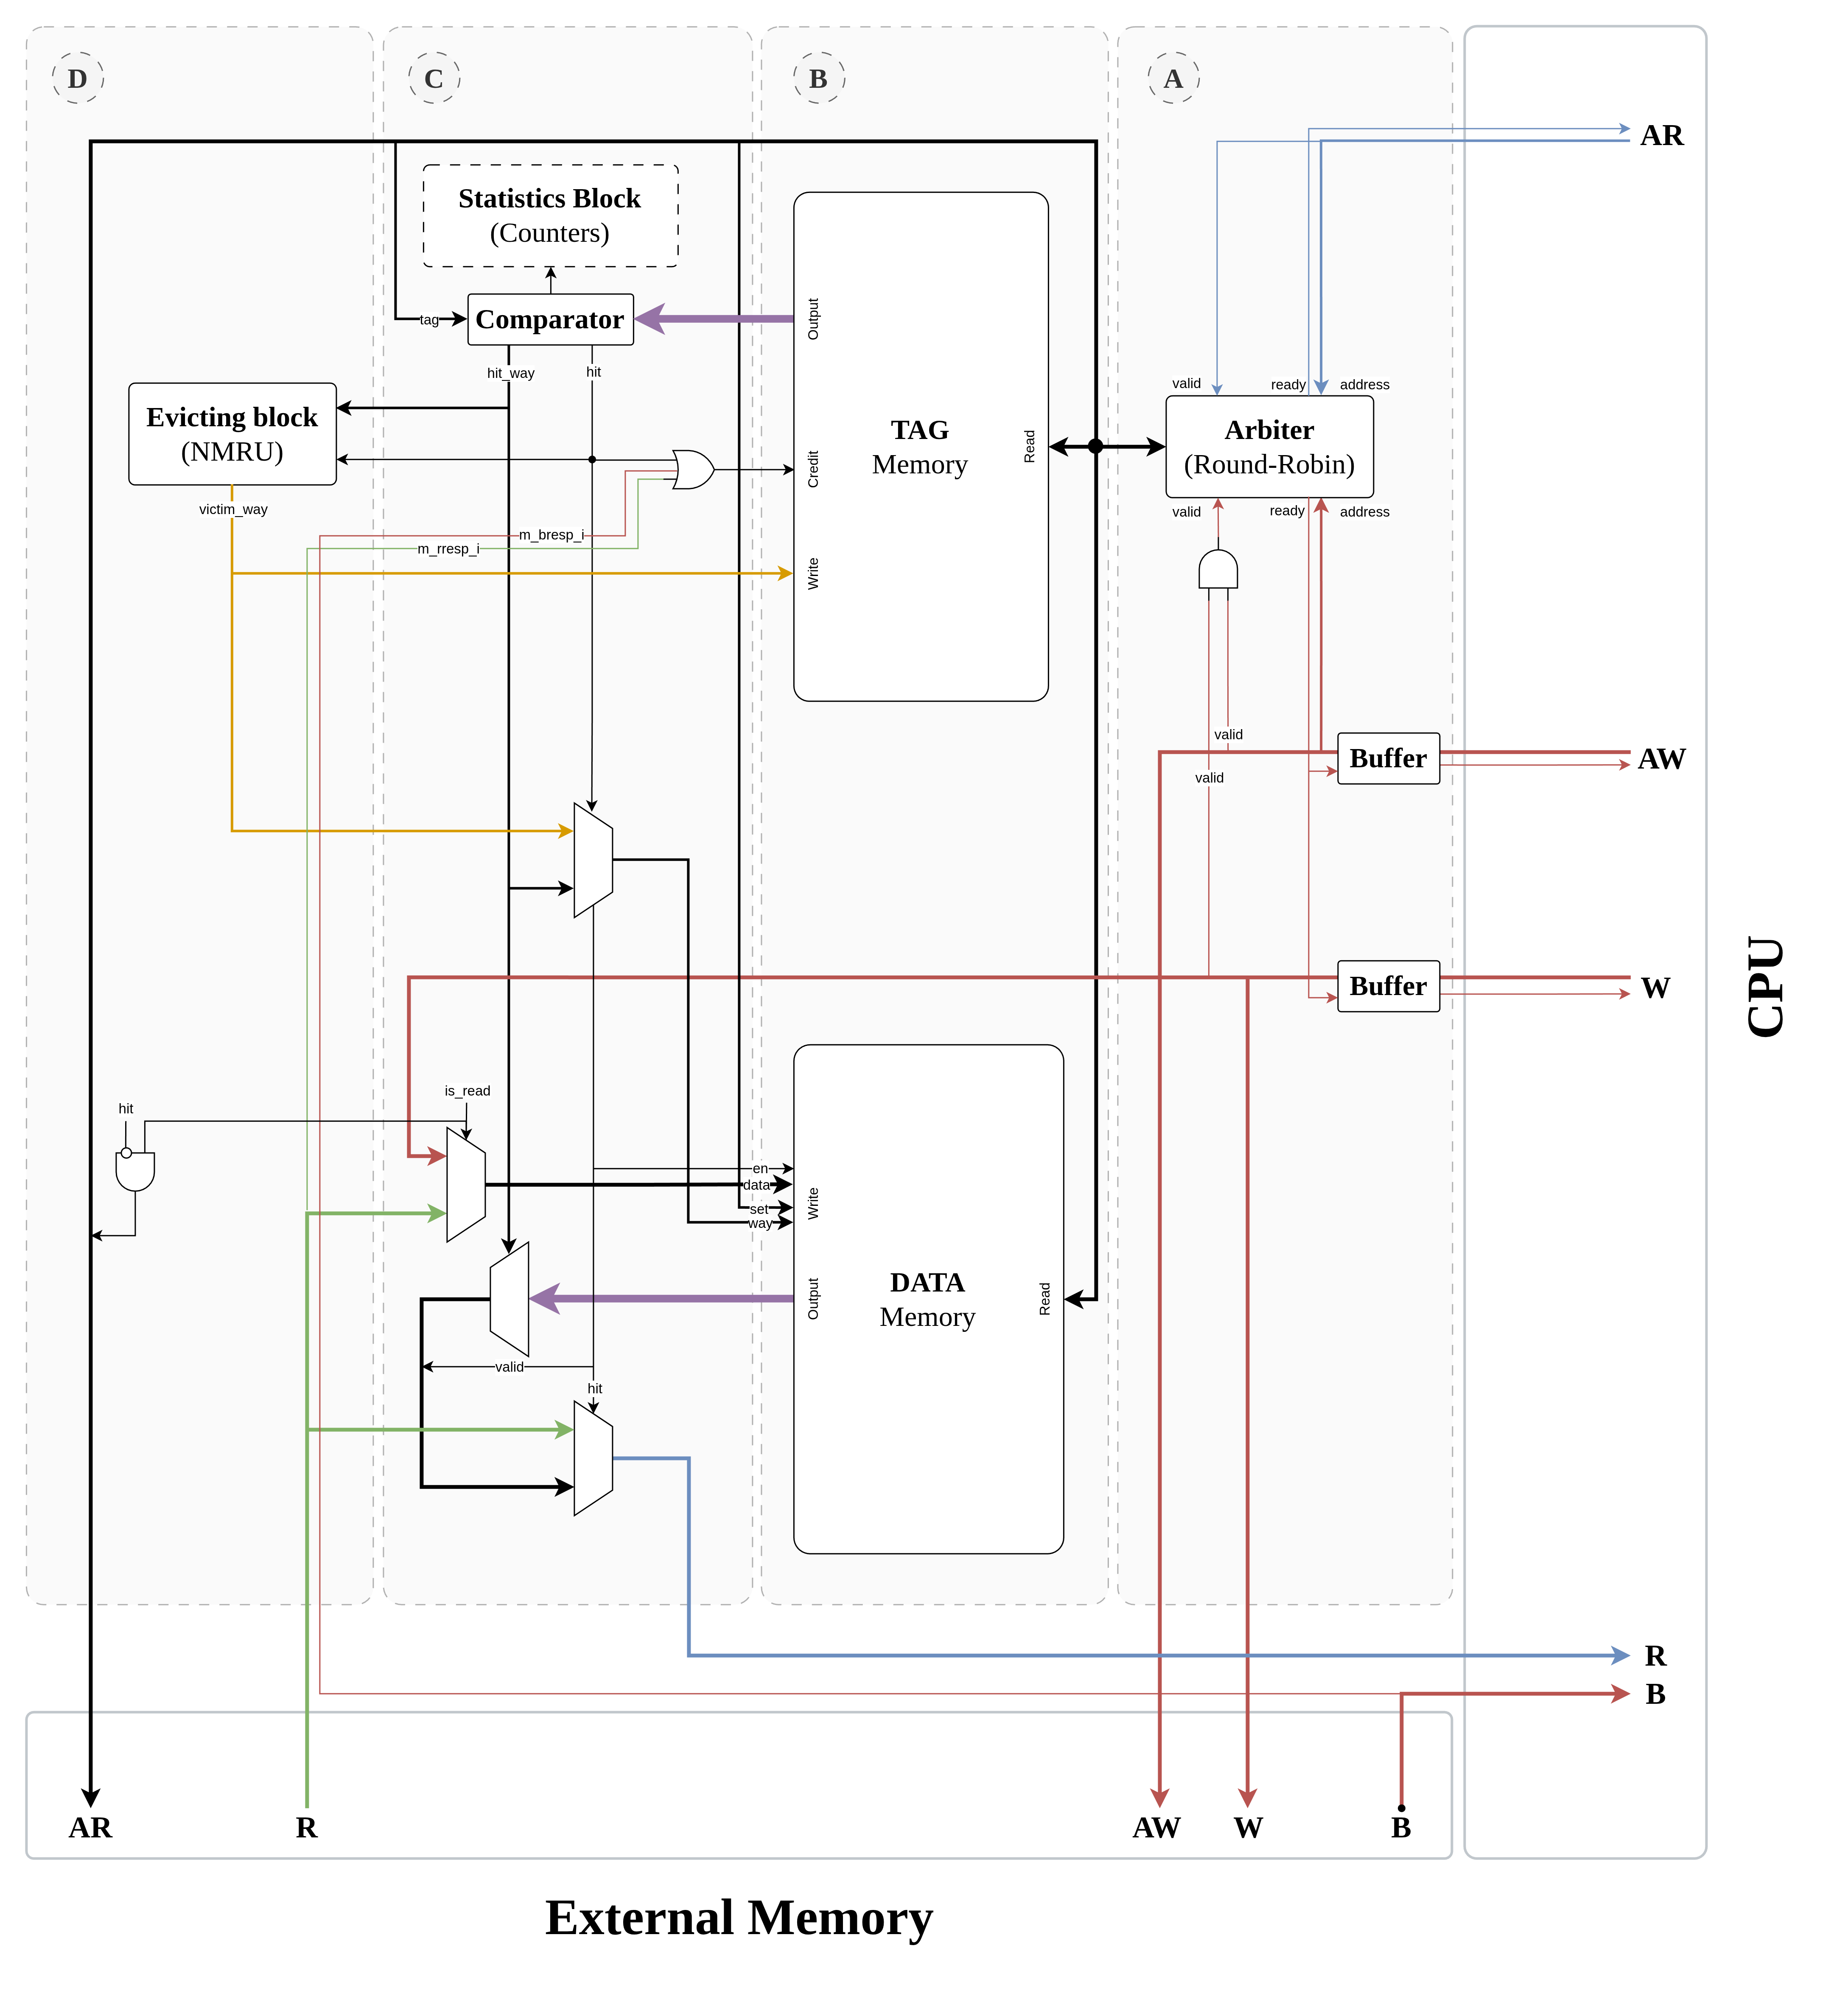
\includegraphics[width=16cm]{Cache.png}
	\caption{Cache scheme}
\end{figure}

\subsection{Request Fetching}

All incoming CPU transactions are initially received by \hyperref[subsec:buffer]{Buffers} located before the \Arbiter. Separate \hyperref[subsec:buffer]{Buffers} are provided for the \verb|AR|, \verb|AW|, and \verb|W| channels (see \circled{A}{fig:cache}).

The \hyperref[subsec:buffer]{Buffers} serve two purposes.
\begin{itemize}
	\item First, they temporarily hold transactions when read and write requests arrive simultaneously, allowing the \Arbiter which operation should be processed first. 
	\item Second, they account for the fact that the \verb|AW| and \verb|W| channels of an AXI4-Lite write transaction may arrive independently and at different times.
\end{itemize}

A write operation is passed to the cache for processing only after both the \verb|AW| and \verb|W| transactions have been received from the CPU.

If only one type of transaction is received, either a read request through the \verb|AR| channel or a complete write request with both \verb|AW| and \verb|W| transactions, it passes through the corresponding buffers and \Arbiter combinatorially.

\subsection{Read Operation}

During a read operation, the CPU provides the requested address through the AXI4-Lite \verb|AR| channel. The address is used simultaneously to initiate a read operation in both the \TagMemory and \DataMemory (see \circled{B}{fig:cache}).

The set index is extracted from the requested address and is used to access the corresponding set in both memories. On the following clock cycle, the \TagMemory provides the tags and valid bits of all ways belonging to the selected set. In parallel, the \DataMemory provides the data stored in all ways of the same set.

The set of ways obtained from the \TagMemory, together with the requested tag extracted from the address, is provided to the \Comparator. The \Comparator compares the requested tag with the tag stored in each way in parallel and determines whether the requested cache line is present (see \circled{C}{fig:cache}). 

\subsubsection{Read Hit}

In case of a cache hit, the \Comparator asserts the hit signal and provides the index of the way containing the requested tag through \verb|hit_way|.

The \verb|hit_way| value is provided to the \EvictingBlock to update the most recently used way for the corresponding set. At the same time, \verb|hit_way| is used to select the required data from the set of ways returned by the \DataMemory. The selected data is then provided to the CPU through the AXI4-Lite \verb|R| channel (see \circled{C}{fig:cache}).

Since the \TagMemory and \DataMemory are accessed in parallel, the cache can determine the requested way and select the corresponding data within a single clock cycle.

\subsubsection{Read Miss}

In case of a cache miss, the \EvictingBlock is activated to select the way that will be replaced in the selected set. The victim way is selected by \PRG while ensuring that the most recently used way is not selected for replacement (see \circled{D}{fig:cache}). The generated victim way is then used to select the cache way that will be overwritten in the \TagMemory.

At the same time, the address of the requested cache line is provided to the external memory through the AXI4-Lite \verb|AR| channel. The data returned by the external memory on the \verb|R| channel is written into the selected way of the \DataMemory and is simultaneously forwarded to the CPU through the CPU-side AXI4-Lite \verb|R| channel (see \circled{C}{fig:cache}).

\subsection{Write Operation}
During a write operation, the data is written directly to the external memory through the AXI4-Lite interface and allocates in the cache according to the write-through policy.

When the CPU provides the write address and data through the AXI4-Lite \verb|AW| and \verb|W| channels, the write address is simultaneously provided to the \TagMemory (see \circled{B}{fig:cache}). The set index extracted from the address is used to access the corresponding set, and the requested tag is compared with the tags of all ways by the \Comparator, following the same procedure as for a read operation (see \circled{C}{fig:cache}).

\subsubsection{Write Hit}

If a matching tag is found, the corresponding way is identified by \verb|hit_way|. The new data is written both to the selected way of the \DataMemory (see \circled{C}{fig:cache}) and to the external memory. The write address and data received from the CPU through the AXI4-Lite \verb|AW| and \verb|W| channels are forwarded to the corresponding channels of the external memory interface.

\subsubsection{Write Miss}

If no matching tag is found, the \EvictingBlock is activated to select the way that will be replaced in the selected set (see \circled{D}{fig:cache}). The victim way is selected by \PRG while ensuring that the most recently used way is not selected for replacement.

The tag of the current write address is written into the selected way of the \TagMemory, and the corresponding data is written into the selected way of the \DataMemory (see \circled{C}{fig:cache}). At the same time, the write address and data received from the CPU through the AXI4-Lite \verb|AW| and \verb|W| channels are forwarded to the corresponding channels of the external memory interface.

\subsection{Hits Counting}
The cache provides hit and miss counting functionality for simulation and performance analysis. This functionality is implemented in the \StatisticsBlock.

The \StatisticsBlock receives hit and miss information from the \Comparator, which determines whether the requested tag is present in the selected cache set.

\begin{infobox}{Simulation Only}
	The \StatisticsBlock is intended exclusively for simulation purposes and is not included in the synthesized cache design. Therefore, it does not introduce any hardware overhead in the final implementation.
\end{infobox}